\begin{algorithm}[!t]
    \caption{Key operations of the N-ary sum tree.}
    \label{alg:n_nary_sum_tree_func}
    \begin{algorithmic}[1]
      \Function{updateValue}{idx, value}
          \State node\_idx = \Call{convertToNodeIdx}{idx};
          \State $\Delta$ = value - \Call{getValue}{node\_idx};
          \While{!\Call{isRoot}{node\_idx}}
              \State new\_value = \Call{getValue}{node\_idx} + $\Delta$;
              \State \Call{SetValue}{node\_idx, new\_value};
              \State node\_idx = \Call{getParent}{node\_idx};
          \EndWhile
      \EndFunction
      \\
      \Function{getPrefixSumIdx}{prefixSum}
          \State node\_idx = \Call{getRoot}{\null};
          \While{!isLeaf(node\_idx)}
              \State node\_idx = \Call{getLeftChild}{node\_idx};
              \State partialSum = 0;
              \For{$i$ = 0; $i$ $<$ fan\_out; $i++$}
                  \State sum = partialSum + \Call{getValue}{node\_idx};
                  \If{sum $\geq$ prefixSum}
                      \State break;
                  \EndIf
                  \State partialSum = sum;
                  \State node\_idx = \Call{getNextSibling}{node\_idx};
              \EndFor
              \State prefixSum = prefixSum - partialSum;
          \EndWhile
          \State idx = \Call{convertToDataIdx}{node\_idx};
          \State \Return idx;
      \EndFunction
    \end{algorithmic}
\end{algorithm}

\section{Parallel Prioritized Replay Buffer}\label{sec:parallel_per}
In this section, we discuss in detail the design of our Prioritized Replay Buffer that supports parallel actors and learners. We start by introducing the key operations that need to be supported.
\subsection{Operations}\label{sec:parallel_per_ops}
\subsubsection{Insertion}
Given a new data item $x$, find the next available index $i$ and insert $x$ at $i$. If the Replay Buffer is full, find the index using the eviction policy. Set the priority at index $i$ to $P(i)=P_{\max}$, where $P(i)$ is the priority at index $i$ and $P_{\max}$ is the maximum priority in the Replay Buffer. The most common eviction policy used in existing implementations is First-in-first-out (FIFO).
\subsubsection{Sampling}
Sample a data item $x_i$ according to the probability distribution $Pr(i)=\nicefrac{P(i)}{\sum_{i}P(i)}, i=1,2,\ldots, N$, where $N$ is the size of the Replay Buffer. To do so, we first sample $x$ from uniform distribution $U(0,1)$. Then, we compute the cumulative density function (cdf) as $cdf(i)=\sum_{j=1}^{i}Pr(j), i=1,2,\ldots, N$. Finally, the sampled index $i=cdf^{-1}(x)$. Mathematically, this is equivalent to finding the minimum index $i$, such that the \textbf{prefix sum} of the probability from 0 to $i$ is greater than or equal to $x$:
\begin{align}
    \min_{i}\sum_{j=1}^{i}Pr(i)\geq x \Rightarrow \min_{i}\sum_{j=1}^{i}P(i)\geq x\cdot \sum_{j=1}^{N}P(j)
    \label{eq:prefix_sum}
\end{align}
\subsubsection{Priority retrieval}
Return the priority at index $i$.
\subsubsection{Priority update}
Update the priority at index $i$.

\subsection{Frequency of the Operations and Runtime Requirements} 
As shown in Algorithm~\ref{alg:off_policy_rl}, the insertion is executed once per iteration. The sampling, priority retrieval and priority update are executed once every update\_interval. Directly storing the priority in an array incurs a runtime complexity of $\Theta(N)$ for sampling and $\Theta(1)$ for priority retrieval and priority update. Directly storing the prefix sum in an array incurs a runtime of $\Theta(\log N)$ in sampling, $\Theta(1)$ in priority retrieval and $\Theta(N)$ in priority update. Based on the frequency of the operations, both these implementations incur a overall runtime complexity of $\Theta(N)$. In this paper, we proposed to use $K$-ary sum tree to implement the Prioritized Replay Buffer to achieve $\Theta(\log N)$ runtime complexity for both sampling and priority update and thus for the entire implementation.

\subsection{$K$-ary Sum Tree}\label{sec:sum_tree}
We show an example of a $K$-ary sum tree for $K=4$ in Figure~\ref{fig:sum_tree}. Each node has $K$ child nodes. The value stored in the parent node is the sum of all the values stored in the child nodes. The leaf nodes hold the actual priorities. 

\begin{figure}
    \centering
    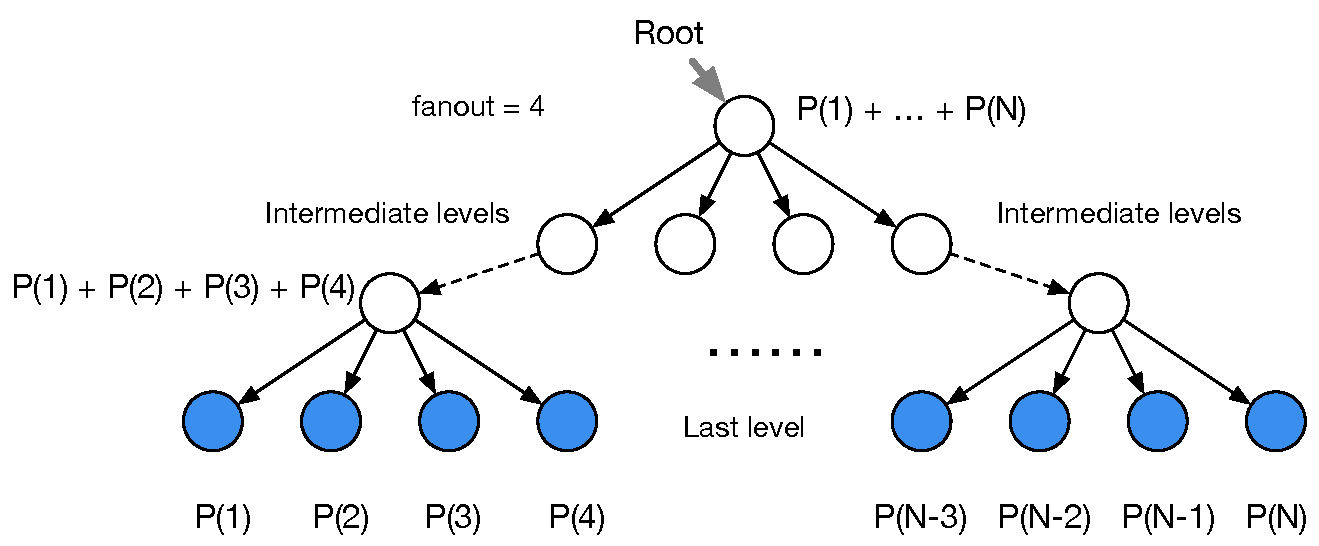
\includegraphics[width=\linewidth]{sum_tree.pdf}
    \caption{The overall structure of a 4-ary sum tree.}
    \label{fig:sum_tree}
\end{figure}

\begin{figure}
    \centering
    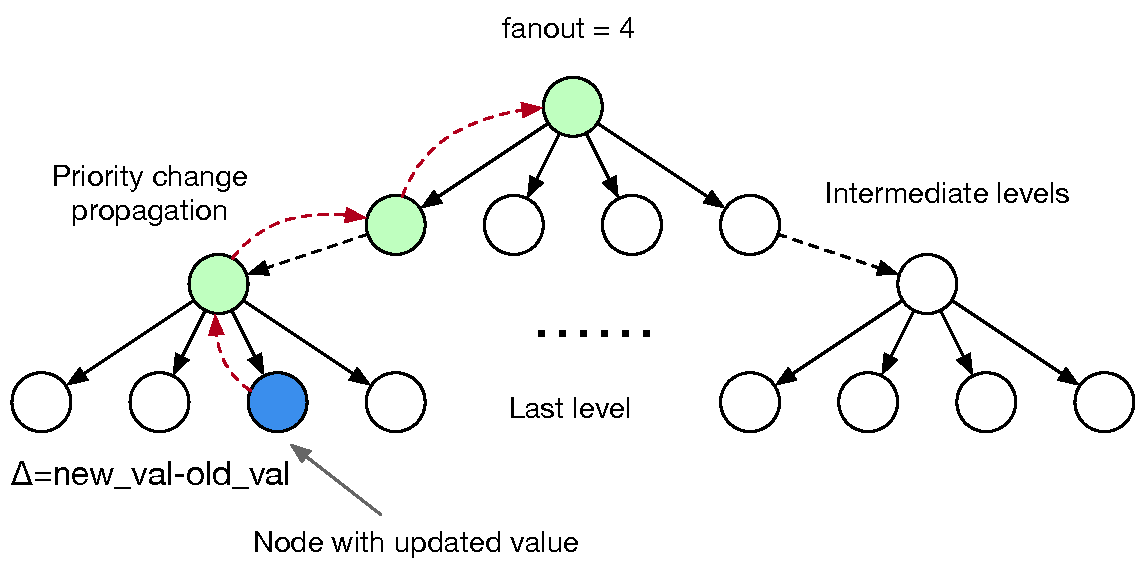
\includegraphics[width=\linewidth]{update_value.pdf}
    \caption{Illustration of the process when updating the value in the $K$-ary sum tree with fanout=4 as shown in Algorithm~\ref{alg:n_nary_sum_tree_func}. The blue node denotes the leaf node that holds the priority. The green nodes denote the intermediate sums that are updated by propagating the change of the priority from the leaf to the root. The red dotted arrow shows the direction of the value propagation.}
    \label{fig:update_value}
\end{figure}

\begin{figure*}
    \centering
    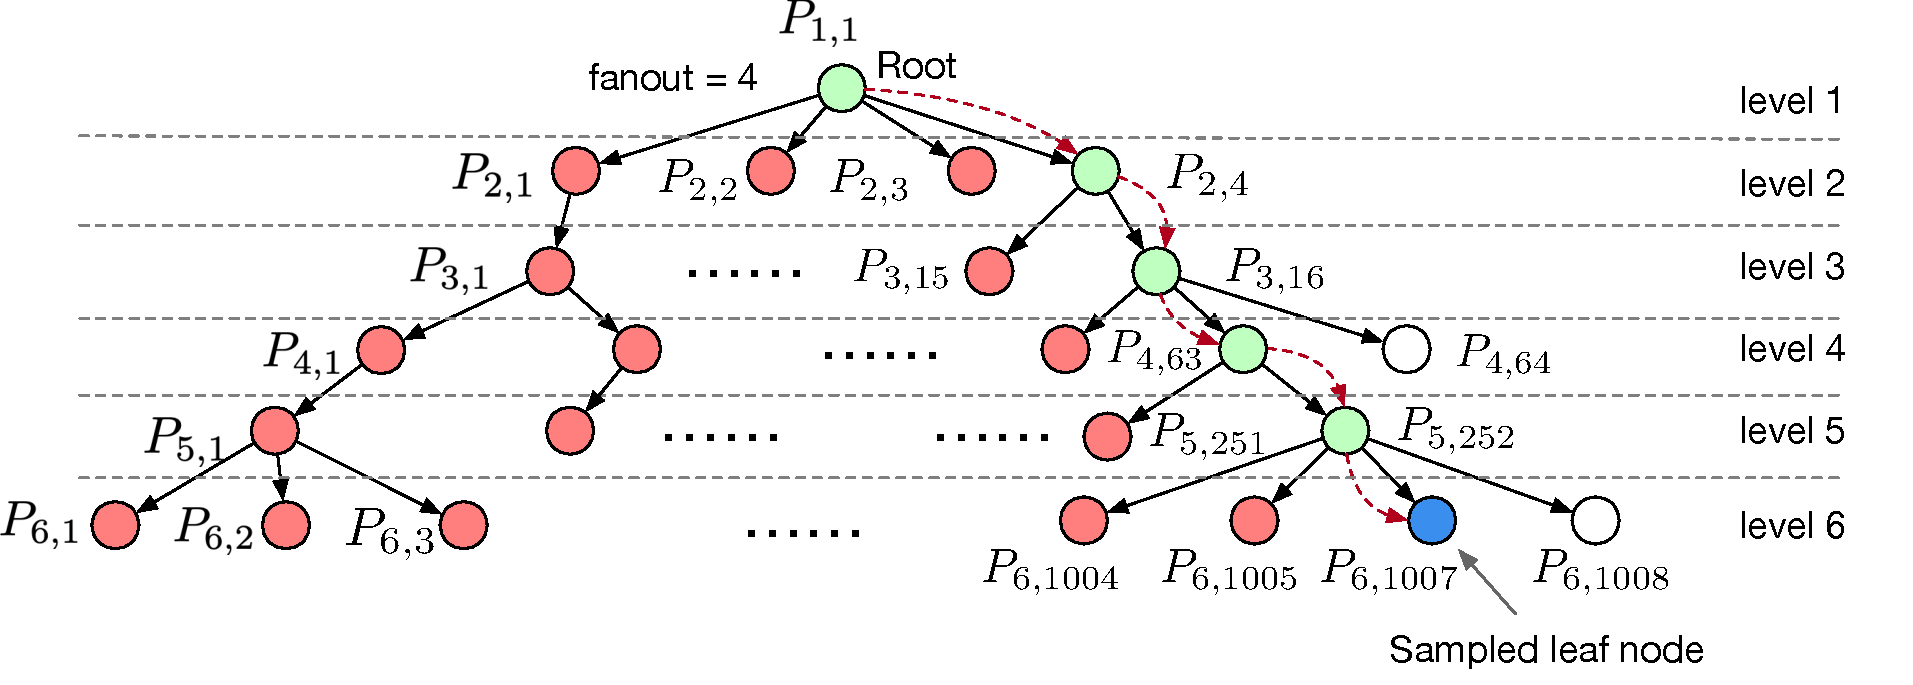
\includegraphics[width=\linewidth]{get_prefix_sum.pdf}
    \caption{Illustration of the process when sampling index according to the priority in the $K$-ary sum tree with fanout=4 as shown in Algorithm~\ref{alg:n_nary_sum_tree_func}. Starting from the root node, the green nodes denote the cutoff node during traversal and the blue node denotes the leaf node sampled. The red dotted arrow shows the direction of the tree traversal.}
    \label{fig:get_prefix_sum}
\end{figure*}

\subsubsection{Priority retrieval}
In order to obtain the priority for the index $i$, we create an array of pointers, each pointing to its corresponding leaf node that holds the priority value. Thus, priority retrieval using $K$-ary sum tree requires $\Theta(1)$ time.

\subsubsection{Priority update}
To update the priority of index $i$, we first obtain the leaf node holding the priority. We compute the change of the priority by subtracting the old value from the new value. Then, we propagate the change of the priority from the leaf node to the root node by traversing along the parent nodes. We show a detailed function in Algorithm~\ref{alg:n_nary_sum_tree_func} and an example in Figure~\ref{fig:update_value}. It is easy to see that this operation requires $\Theta(\log_K N)$ time.

\subsubsection{Prefix sum index computation}
Given a randomly sampled number $x\sim U(0,1)$, the objective is to compute index $i=\min_{i}\sum_{j=1}^{i}P(i)\geq x\cdot \sum_{j=1}^{N}P(j)$ as discussed in Section~\ref{sec:parallel_per_ops}. The sum of all the priorities in the Replay Buffer $\sum_{j=1}^{N}P(j)$ can be computed in $\Theta(1)$ by simply retrieving the value stored in the root node. To design an algorithm that obtains the target index, we start by proving Lemma~\ref{lemma:index_existence} and theorem~\ref{the:sum_tree_prefix}:

\begin{lemma}
    \label{lemma:index_existence}
    Let the value of the $i$-$th$ node at level $m$ be $P_{i,m}$. Assume the height of the tree is $H$. Then, at level $1\leq m\leq H$, there exists index $j$, $1 \leq j \leq K^{m-1}$, such that $\sum_{i=1}^{j}P_{m, i}\geq x\cdot \sum_{i=1}^{N}P(i)$, for any $x\in (0, 1)$.
\end{lemma}
\begin{proof}
    According to the definition, the leaf node holds the priority value. Thus, $P_{i, H}=P(i), \forall i=1,2,\ldots, K^{H-1}$. Since $x\in (0, 1)$, we obtain $x\cdot \sum_{i=1}^{N}P(i)\leq \sum_{i=1}^{N}P(i) \leq \sum_{i=1}^{K^{H-1}}P_{i,H}$. Because the priority values are non-negative, there must exist index $j$, $1 \leq j \leq K^{H-1}$, such that $\sum_{i=1}^{j}P_{H, i}\geq x\cdot \sum_{i=1}^{N}P(i)$. According to the property of the sum tree, the value of the parent is the sum of all its children. Thus, $\sum_{i=1}^{K^{H-1}}P_{H, i}=\sum_{i=1}^{K^{m-1}}P_{m, i}, \forall m=1, 2, \cdots, H-1$. Therefore, the same argument holds for each level. This concludes the proof for Lemma~\ref{lemma:index_existence}.
\end{proof}
\begin{theorem}
    \label{the:sum_tree_prefix}
    Let $j_m=\min_{j'} \sum_{i=1}^{j'}P_{m, i}\geq x\cdot \sum_{i=1}^{N}P(i)$. Then, $j_m$ is the parent node of $j_{m+1}$, $\forall m=1,2,\cdots H-1$.
\end{theorem}
\begin{proof}
    The child nodes of index $j$ at level $m$ are $K\cdot(j-1)+1,\cdots, K\cdot j$ at level $m+1$. According to the definition of the sum tree and the property of $j_m$, we obtain $\sum_{i=1}^{j_m-1}P_{m,i}=\sum_{i=1}^{K\cdot(j_m-1)}P_{m+1, i}< x\cdot \sum_{i=1}^{N}P(i)$. Thus, the index of the cutoff node at level $m+1$ must be $j_{m+1}\geq K\cdot(j_m-1)+1$. Noticing that $\sum_{i=1}^{j_m}P_{m,i}=\sum_{i=1}^{K\cdot(j_m)}P_{m+1, i}\geq x\cdot \sum_{i=1}^{N}P(i)$. Thus, the index of the cutoff node at level $m+1$ satisfies $j_{m+1}\leq K\cdot j_m$. Combining $K\cdot(j_m-1)\leq j_{m+1}\leq K\cdot j_m$, we obtain $j_m$ is the parent node of $j_{m+1}$.
\end{proof}
We refer such node $j_m$ as the \textit{cutoff node} at level $m$. The goal of sampling is to find the index of the cutoff node at the last level of the tree. 
According to Theorem~\ref{the:sum_tree_prefix}, the cutoff node at level $m$ is the parent of the cutoff node at level $m+1$. 
Therefore, we can start from the root node and perform the search only using the child nodes. To obtain which child node is the cutoff node, we maintain a cumulative sum of all the nodes left to the cutoff at each level. Please refer to Algorithm~\ref{alg:n_nary_sum_tree_func} for details.
We also illustrate an example of the process in Figure~\ref{fig:get_prefix_sum}, where $K=4$ and $H=6$.

\subsubsection{Data layout}
Maintaining the explicit tree data structure using pointers significantly degrades the cache performance of modern CPUs. In this work, we implement the tree data structure implicitly using an array as shown in Figure~\ref{fig:data_layout}. The sampling process requires traversing all the nodes under the same parent. To maximize the cache performance, it is desired that each group of child nodes under the same parent is cache aligned. Assume that one cacheline can store $C$ nodes, then we choose $K$, such that $K\%C=0$. We pad the root node with $K-1$ so that it is also cache aligned.

\begin{figure}
    \centering
    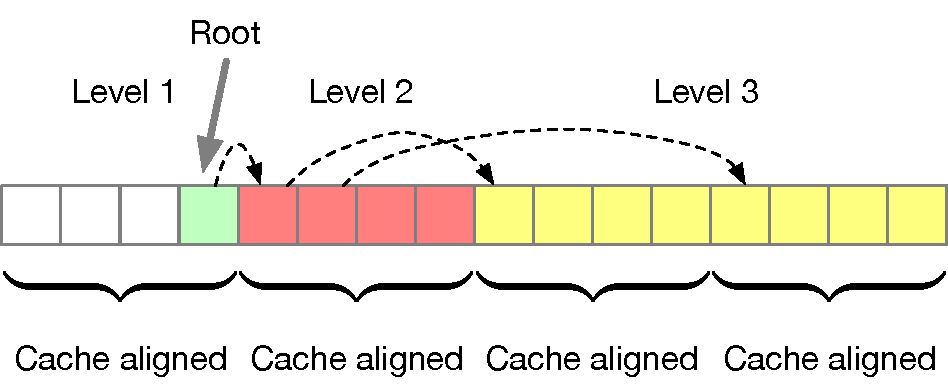
\includegraphics[width=\linewidth]{data_layout.pdf}
    \caption{Data layout of the proposed sum tree with $K=4$. The black arrow shows the first child of the parent node. The color indicates the level of the node in the tree.}
    \label{fig:data_layout}
\end{figure}

\subsubsection{Theoretical performance analysis}
\paragraph{Space complexity}
The space complexity is proportional to the number of nodes in the tree. Assume the size of the Replay Buffer is $N$, which is equal to the number of nodes in the last level of the tree. Thus, the total number of nodes in the tree is: $\Theta(\frac{K^H-1}{K-1})=\Theta(\frac{K^{H-1}\cdot K-1}{K-1})=\Theta(\frac{N\cdot K-1}{K-1})=\Theta(N+\frac{N-1}{K-1})$. Clearly, as $K$ increases, the space complexity reduces due to the decrease of the number of intermediate nodes.

\paragraph{Runtime complexity}
It is clear that the priority retrieval runs in $\Theta(1)$ and priority update runs in $\Theta(\log_K N)$. For prefix sum index computation, the loops runs $H=\ceil{\log_K N} + 1$ times. The memory access inside loop has $\nicefrac{K}{C}$ cache misses and $K\cdot(1-\nicefrac{1}{C})$ cache hit, where $C$ is the number of nodes in one cacheline. Thus, the time complexity of prefix sum index computation is $\Theta((\log_K N+1)(T_{miss}\cdot\frac{K}{C}+T_{hit}\cdot K\cdot(1-\nicefrac{1}{C})))$, where $T_{miss}$ is the execution time of one cache miss and $T_{hit}$ is the execution time of one cache hit. Note that this function has a local minimum in terms of $K$. In practice, we profile the performance of various $K$ values based on the size of the cacheline and choose the one that yields the best performance.

\subsection{Thread-safe Prioritized Replay Buffer}\label{sec:thread_safe_prb}
In order to support parallel actors and learners, it is crucial to design thread-safe prioritized Replay Buffer. We summarize the resource utilization of various operations in Table~\ref{table:resource_util}. We design the thread-safe prioritized replay buffer using locking mechanism such that the duration of holding a lock is minimized. 

\subsubsection{Synchronization of the sum tree}
We use two locks to synchronize the sum tree: one to synchronize the read/write of the last level of the tree and the other to synchronize the read/write of all the levels. A detailed procedure of priority update and priority retrieval is shown in Algorithm~\ref{alg:sync_replay_buffer}. Using this technique, reading of the priority value and updating of the intermediate levels of the sum tree can be executed in parallel. Note that it will cause inconsistencies if we acquire the global\_tree\_lock after releasing the last\_level\_lock lock when two priority update queries arrive at the same time.

\subsubsection{Synchronization of insertion and sampling}
During insertion, the Replay Buffer finds an available index. Then, it writes the data to the storage and updates the priority to the maximum priority in the Replay Buffer. Compared with index searching and priority update, data writing takes more time due to explicit copy of the memory data. Thus, it is important not to hold the lock while performing the data writing. To do so, we propose \textit{lazy writing}: 1) We set the priority to zero atomically; ii) we perform data writing; iii) we reset the priority to the maximum priority in the Replay Buffer atomically. Since the priority is zero during data writing, it will never be sampled. This makes sampling only needs to synchronize prefix sum index computation. A detailed procedure is shown in Algorithm~\ref{alg:sync_replay_buffer}.


\begin{algorithm}[!t]
    \caption{Synchronization of the Prioritized Replay Buffer}
    \label{alg:sync_replay_buffer}
    \begin{algorithmic}[1]
        \Function{PriorityUpdate}{idx, new\_priority}
            \State \Call{Acquire}{global\_tree\_lock};
            \State \Call{Acquire}{last\_level\_lock};
            \State \Call{UpdateLastLevel}{\null};
            \State \Call{Release}{last\_level\_lock};
            \State \Call{UpdateIntermediateLevel}{\null};
            \State \Call{Release}{global\_tree\_lock};
        \EndFunction
        \\
        \Function{PriorityRetrieval}{idx}
            \State \Call{Acquire}{last\_level\_lock};
            \State priority = \Call{getPriority}{idx};
            \State \Call{Release}{last\_level\_lock};
            \State \Return priority;
        \EndFunction
        \\
        \Function{Insert}{idx, data}
            \State \Call{UpdatePriority}{idx, 0};
            \State \Call{WriteToStorage}{idx, data};
            \State \Call{UpdatePriority}{idx, max\_priority};
        \EndFunction
        \\
        \Function{Sample}{\null}
            \State \Call{Acquire}{global\_tree\_lock};
            \State idx, priority = \Call{getPrefixSumIndex}{\null};
            \State \Call{Release}{global\_tree\_lock};
            \State \Return idx, priority;
        \EndFunction
    \end{algorithmic}
\end{algorithm}


\begin{table}[!t]
    \centering
    \caption{Resource utilization of various operations}
    \vspace{-1em}
    \begin{tabular}{cc}
        \toprule
        Operations & Resource Utilization  \\
        \midrule
        Insertion & modify the entire tree, modify the storage \\
        Sampling & access the entire tree, access the storage \\
        Priority retrieval & access the last level of the tree \\
        Priority update & modify the entire tree \\
        \bottomrule
    \end{tabular}
    \label{table:resource_util}
\end{table}

\subsubsection{Write after read vs. read after write}
The parallelism of the priority update and the data sampling causes data dependency issues: the same data is sampling using the old priority before the new priority gets updated (write after read). Mathematically, only read after write is valid and write after read produces inconsistent results. However, it has little impact in practice as neural network training is stochastic in nature and robust to such transient inconsistencies.
